\chapter{Introduction to PHAISTOS}

This section servers as an introduction to the PHAISTOS program, and a (very) brief introduction to the theory behind PHAISTOS\cite{Phaistos}. 
This will give the relevant background to read the next chapters.
PHAISTOS is also published and discussed in detail in paper \#2 in this the appendix.

\section{Markov Chain Monte Carlo}

One of the primary goals of simulations in PHAISTOS is to construct the Boltzmann distribution of a protein via Markov chain Monte Carlo (MCMC) sampling for a given potential energy surface at a given temperature.
The Boltzmann distribution of a protein structure, $\mathbf X$, at a given temperature, $T$, is given by:
\begin{equation}
    \label{eq:boltzmann}
    p(\mathbf X) = \frac{1}{Z(T)} \exp{\left( \frac{-E}{k_\mathrm{B}T}\right)},
\end{equation}
where $k_\mathrm{B}T$ is Boltzmann's constant and $Z(T)$ is the partition function at the given temperature.

In Markov chain Monte Carlo the target distribution obtained by repeatedly proposing updates to the current state, and accepting or rejecting these updates with a certain acceptance probability.

It can be shown, that for an infinitely sampled distribution to converge to the correct target distribution, i.e.~$p_\infty(\mathbf X) = p(\mathbf X)$, the Monte Carlo moves that are used to propose updates must satisfy the principle of detailed balance.
That is, the transition from the current state $\mathbf{X}$ to the proposed new state $\mathbf{X'}$ fulfills:
\begin{equation}
    \label{eq:detailed_balance}
    p(\mathbf{X}) p(\mathbf{X} \rightarrow \mathbf{X'}) = 
    p(\mathbf{X'}) p(\mathbf{X'} \rightarrow \mathbf{X})
\end{equation}
where $p(\mathbf{X} \rightarrow \mathbf{X'})$ is the probability to of moving from the state $\mathbf{X}$ to $\mathbf{X'}$ using a given move.
If we further factorize $p(\mathbf{X} \rightarrow \mathbf{X'})$ into an acceptance probability $p_a$ and a move transition probability $p_m$, Eqn. \ref{eq:detailed_balance} gives:
\begin{equation}
    \label{eq:unbiased_mc}
    \frac{p_a(\mathbf{X} \rightarrow \mathbf{X'})}
         {p_a(\mathbf{X'} \rightarrow \mathbf{X})} =
    \frac{p(\mathbf{X'})}
         {p(\mathbf{X})}
    \frac{p_m(\mathbf{X'} \rightarrow \mathbf{X})}
         {p_m(\mathbf{X} \rightarrow \mathbf{X'})}
\end{equation}
Most of the moves in PHAISTOS are symmetric, that is the move bias ratio $p_m(\mathbf{X'} \rightarrow \mathbf{X}) / p_m(\mathbf{X} \rightarrow \mathbf{X'}) = 1$, but for some moves this is not true. 
These biased moves can be exploited to vastly speed up convergence or bias the simulation, and are discussed later in Section \ref{chap:generative}.

\subsection{Metropolis-Hastings}
The simplest Monte Carlo method that satisfies Eqn.~\ref{eq:unbiased_mc} is the Metropolis-Hastings method.
Here a transition $\mathbf{X} \rightarrow \mathbf{X'}$ is accepted using the Metropolis-Hastings acceptance criterion:
\begin{equation}
    \label{eq:mc_mh}
    p_a(\mathbf{X} \rightarrow \mathbf{X'}) = \min \left( 1,
    \frac{p(\mathbf{X'})}
         {p(\mathbf{X})}
    \frac{p_m(\mathbf{X'} \rightarrow \mathbf{X})}
         {p_m(\mathbf{X} \rightarrow \mathbf{X'})} \right)
\end{equation}
%Note how the term $1/Z(T)$ term from Eqn.~\ref{eq:boltzmann} cancels out.
Evaluation of the partition function is thus not necessary.
The Metropolis-Hastings method is efficient when exploring native states, and simulations near the critical temperature.
Unfortunately the Metropolis-Hastings method, compared to other MC methods, often gets stuck in local minima, and is therefore generally inefficient when simulating protein folding from an extended strand.

\subsection{Generalized Ensembles}
To avoid the slow convergence problem advanced MC methods are available in PHAISTOS, which emphasize sampling at low energies, which is generally of higher interest in protein structure determination.
These "generalized ensemble" methods are very similar to the Metropolis-Hastings method, and the main difference in the acceptance criterion is that the target distribution $p(\mathbf{X})$ has been replace by a generalized weight function $w(\mathbf{X})$. 
The acceptance criterion then becomes:
\begin{equation}
    \label{eq:mc_gh}
    p_a(\mathbf{X} \rightarrow \mathbf{X'}) = \min \left( 1,
    \frac{w(\mathbf{X'})}
         {w(\mathbf{X})}
    \frac{p_m(\mathbf{X'} \rightarrow \mathbf{X})}
         {p_m(\mathbf{X} \rightarrow \mathbf{X'})} \right)
\end{equation}
Through reweighting, samples from a converged simulation in a generalized ensemble can be reweighted to correspond to the Boltzmann distribution at a given temperature.

PHAISTOS offer two generalized ensemble methods.
In the multicanonical ensemble method, the weight function is $w_\mathrm{muca}(\mathbf{X}) = 1/g(E(\mathbf{X}))$, where $E(\mathbf{X})$ is the energy of the structure $\mathbf{X}$ and $g$ is the associated density of states.
In the inverse-$k$ ensemble, the weight function is given by $w_\textit{1/k}(\mathbf{X}) = 1/k(E(\mathbf{X}))$ where $k(E(\mathbf{X})) = \int_{-\infty}^{E(\mathbf{X})} g(E') dE'$.
The since the density of states is generally unknown, the weight-function is estimated during the simulation.
PHAISTOS uses the MUNINN library to collect histograms of the energy and efficiently provide an estimate of $w(\mathbf{X})$ on-the-fly \cite{muninn}.


\section{Monte Carlo Moves Using Generative Probabilistic Models}
\label{chap:generative}
PHAISTOS proposes new structure samples using a weighted set of difference MC moves, which each randomly changes the current protein structure in a certain way. Briefly, these are divided in side chain moves and backbone moves.
Side chain moves update the rotamer-conformation of a amino-acid single side chain by rotating the dihedral angles on the side chain.
Backbone moves either perform a local perturbation to a strand of a only a few amino acids, or rotates one dihedral angle on the backbone.
\\\\Using random moves which re-sample angles from a uniform distribution, and then constructing a target distribution via an acceptance criterion is a perfectly valid strategy.
However, sampling from a uniform distribution usually lead to slow convergence.
A common approach to alleviate this problem is using fragment assembly, in which small fragments of peptides are assembled from a library of common fragment motifs, such as beta-strands, helices and loops.
This approach, however, introduces a move bias, which must be divided out if the simulation has to obey detailed balance.
Furthermore, it is not clear, how to evaluate the move bias ratio $p_m(\mathbf{X'} \rightarrow \mathbf{X}) / p_m(\mathbf{X} \rightarrow \mathbf{X'})$ when sampling from a fragment library.

A related approach to obtain a similar speed up is biased sampling.
PHAISTOS supports sampling of both side chain and backbone angles from such generative probabilistic models.
In this approach, angles are sampled from distributions that are conditioned on prior knowledge.
Two all-atom generative probabilistic models are supported in PHAISTOS.
TorusDBN which is a hidden-Markov model of backbone angles\cite{Torus08}, and BASILISK\cite{BASILISK} which is a similar model of side chain rotamer-conformations.
Both work are continuous models in torsion-angle space.
The model that is used in this work is TorusDBN, which is is a model that samples backbone dihedral angles conditioned on the amino acid sequence from a distribution that resembles the Ramachandran-plot.
This effectively speeds up convergence of sampling, since uninteresting parts of conformational space in only sampled very rarely.
The importance of the TorusDBN model is discussed in chapter \ref{chapter:results}.

Using models such as TorusDBN and BASILISK introduces a move bias, which compensated for in Eqn.~\ref{eq:unbiased_mc} by multiplying by the ratio $p_m(\mathbf{X'}     \rightarrow \mathbf{X}) / p_m(\mathbf{X} \rightarrow \mathbf{X'})$.
It is possible to determine this ration, because the likelihood of sampled values can be calculated in the TorusDBN model.
It is thus possible, to recover the target distribution (e.g.~the Boltzmann distribution or a generalized ensemble), despite using only biased moves.


Effectively, this turns the target distribution into an effective target distribution.
For sampling from the Boltzmann distribution (e.g.~using a molecular mechanics force field), the effective target distribution becomes
\begin{equation}
    p_e(\mathbf{X}) = p(\mathbf{X}) p_{m}(\mathbf{X}|I),
\end{equation}
where $p_{m}(\mathbf{X}|I)$ is the probability distribution from the generative model, conditioned on the prior information $I$ available to the model.
This is approach is formally equivalent to adding the term $\ln{(p_{m}(\mathbf{X}|I))}$ to the physical energy (although this term does not scale with the temperature):
\begin{eqnarray}
    p_e(\mathbf{X})
    &=& p(\mathbf{X}) p_{m}(\mathbf{X}|I) \nonumber\\
    &\propto& \exp{\left( \frac{-E(\mathbf{X})}{k_{\mathrm{B}}T} \right)}p_{m}(\mathbf{X}|I) \nonumber\\
    &\propto& \exp{\left( \frac{-E(\mathbf{X})}{k_{\mathrm{B}}T} - \ln{(p_{m}(\mathbf{X    }|I))}\right)}
%    &=& \exp{\left( \frac{-( E(\mathbf{X}) + k_{\mathrm{B}}T \ln{(p_{m}(\mathbf{X}|I))}}{k_{\mathrm{B}}T}\right)}
\end{eqnarray}
In other words, biased sampling can be regarded as simply use of a better force field, while the convergence of the simulation is vastly improved.

TorusDBN is implemented in two versions;
standard TorusDBN which, in brief, is conditioned on only the amino-acid sequence, and TorusDBN-CS which is furthermore based on backbone and beta-carbon chemical shifts.
The default TorusDBN model is trained on a set of 1,447 proteins of 180 different SCOP-fold classifications. 
The default TorusDBN-CS model is trained on 1349 proteins and corresponding chemical shifts from the RefDB training set.

Effectively, proposing structures from TorusDBN biases the simulation towards likely angles within the Ramachandran-plot, and furthermore also towards a certain secondary structure type that is likely for the particular amino acid sequence.
The effect of TorusDBN-CS is similar, but the effect is much more pronounced.

Fig.~\ref{fig:torus} shows an example of three different, but typical cases from Ubiquitin. These are alpha-helix, beta-sheet and loop regions.
Residue 29 (lysine) is in a typical alpha helix and this corresponds to the most often sampled cluster from both TorusDBN and TorusDBN-CS. TorusDBN-CS, however, very precisely locates the center of the cluster to within around $\pm 15$ degrees. TorusDBN, in contrast, has some sampling density in the regions typical for beta-sheet and left-handed alpha-helices.

For residue 44 (isoleucine) which is in a typical alpha-helix region of Ubiquitin, TorusDBN-CS accurately pinpoints the distribution of samples around the experimental values.
TorusDBN, however, manages to rule out left-handed helices, but has a higher sampling density in the alpha-helix region than the beta-sheet region. 

The last residue in the examples, residue 60 (aspargine), is located in a loop-region with backbone angles that correspond to a left-handed helix.
Both models sample in the correct region, but TorusDBN favor a regular alpha-helix.
While TorusDBN-CS heavily favors the correct region, angles that are usually not favored in the Ramachandran plot are also frequently sampled in this particular case.
This is presumably due to less fold-diversity in the training set, compared to the set used to train TorusDBN. Generally, however, the TorusDBN-CS distribution is more restrictive than standard TorusDBN.

\begin{figure}
    \centering
    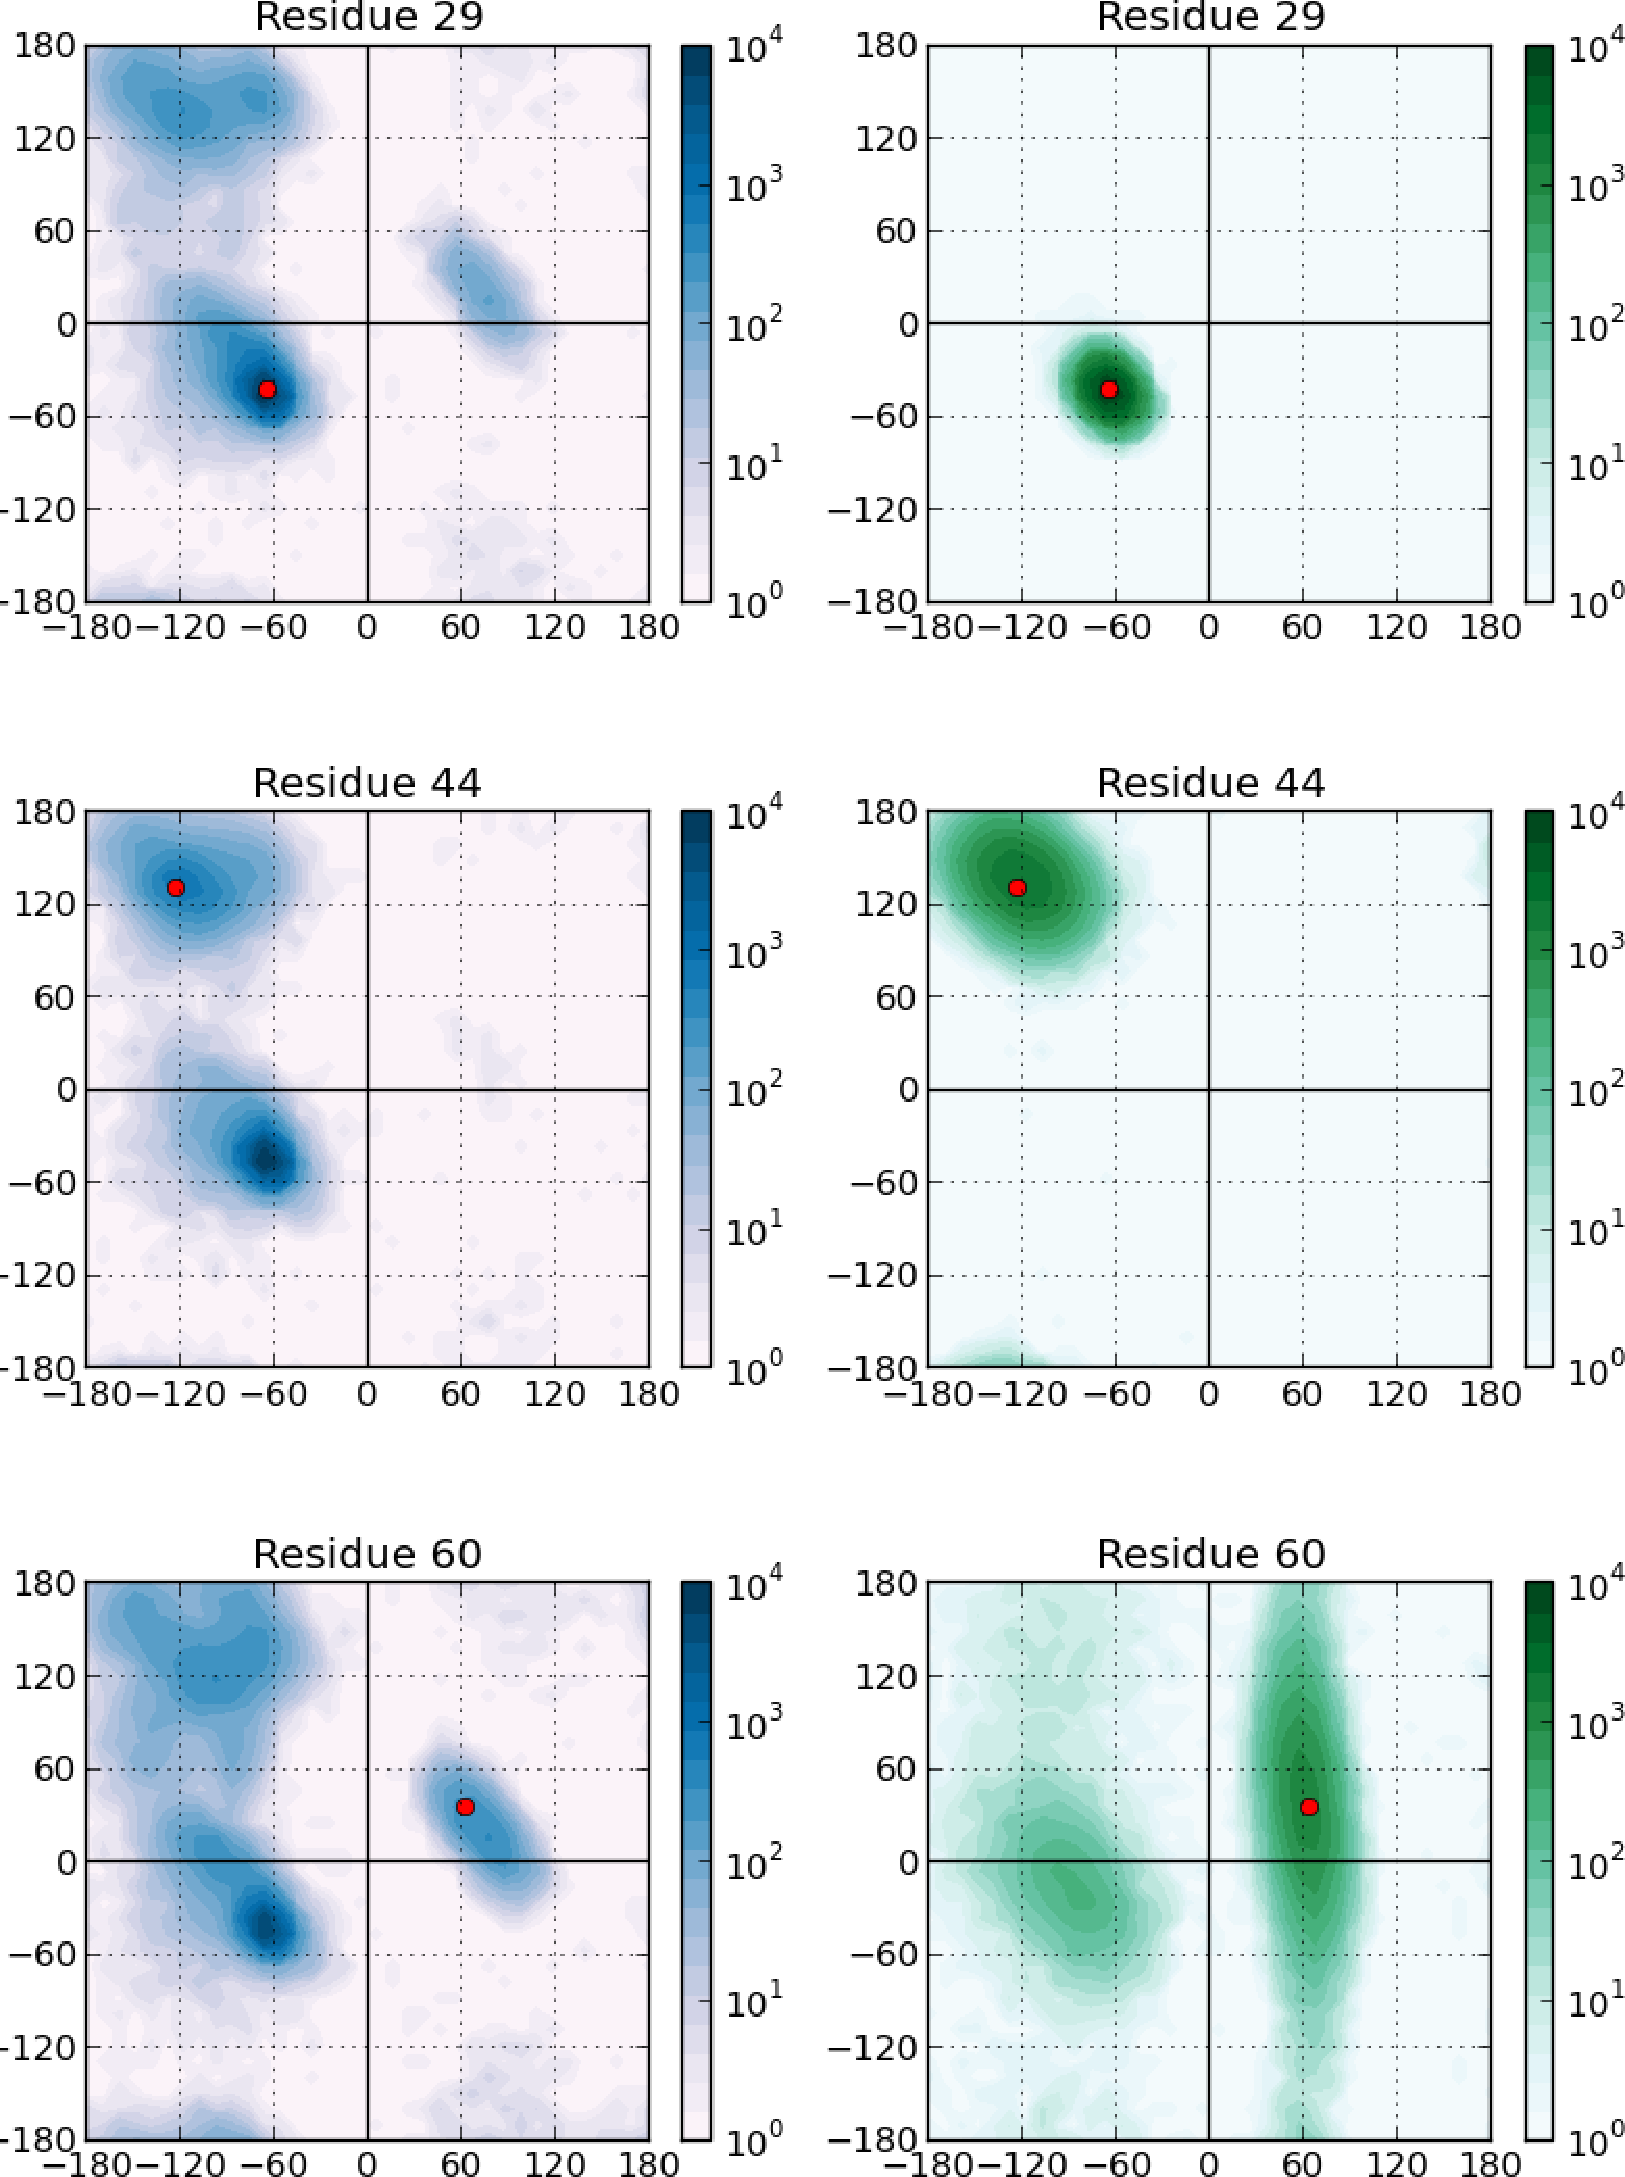
\includegraphics[width=0.75\textwidth]{figures/torus_versions.pdf}
    \caption{Sampling densities from TorusDBN (left/blue) and TorusDBN-CS (right/green) for the residues 29, 44 and 60 in Ubiquitin. Values from the experimental structure 1UBQ are marked with a red dot. Residue 29 (lysine) is located in the middle of an alpha-helix. Residue 44 (isoleucine) is located in a beta-sheet motif, and finally residue 60 (aspargine) is located in a loop region.}
    \label{fig:torus}
\end{figure}

\subsection{Monte Carlo Moves}

PHAISTOS explores the conformational space by applying local Monte Carlo moves to the protein structure.
Moves are divided into backbone and side chain moves.
All moves work by perturbing one or more internal coordinates.
In principle, all internal coordinates are degrees of freedom.
However, since bond angles and bond lengths are not treated explicitly by the PROFASI force field, these are constrained by the MC moves to standard values \cite{engh-huber}
Effectively, only dihedral angles are degrees of freedom in the simulations presented here.

This constraint can of course be lifted if the force field include appropriate terms to describe bond angles and bond lengths.
For instance this is supported by the OPLS-AA/L force field included in PHAISTOS, which was used in Paper \#3.


Three different move-types are used in the simulations presented later in this work.
These are introduced below.
\subsubsection{Pivot Move}
The pivot move re-samples one dihedral angle of the protein backbone. This usually cause large perturbations since two parts of the protein are rotated relative to each other.
As demonstrated later, it is, however, very efficient guiding a folding simulation when biased re-sampling is carried out through TorusDBN or TorusDBN-CS \cite{Torus08}.

\subsubsection{CRISP Move}
In the CRISP move, a number of consecutive residues are selected (default is 7), and the backbone angles of these are perturbed under the constraint that the end-points are fixed in space \cite{crisp}.
This move is particularly efficient at exploring dense states, such as native and near-native states.
This move also supports biased sampling from TorusDBN and TorusDBN-CS.

\subsubsection{Side chain Move}
Side chain moves can either sample new angles uniformly or biased from via BASILISK \cite{BASILISK}.
Additionally, side chain conformations can be drawn from the Dunbrack-rotamer library \cite{dunbrack}.


% \section{Note on protein Folding}
% While converged sampling of the potential energy surface will corresponds to the Boltzmann distribution, and the native folded state of the protein will usually correspond to the largest populated cluster of samples.
% 
% However, due to practical limits on computational resources, it is generally impossible to perform converged sampling of the potential energy surface.
% Protein folding simulations from an extended strand will often be very far from convergence.
% 
% An often used strategy is to determine a structure by selecting the structure with the lowest energy throughout a simulation.
% This obviously neglects entropic effect which may be very important in certain cases, but in practice this has shown to be a very efficient strategy to determine structures close to those obtained experimentally. [REF XX]
% 

